\documentclass[10pt,conference,compsocconf]{IEEEtran}

\usepackage{hyperref}
\usepackage{graphicx}	% For figure environment
\usepackage{amssymb}
\usepackage{authblk}
\usepackage{color}
\usepackage{graphicx}
\graphicspath{ {images/} }
\usepackage[skip=2pt]{caption} % example skip set to 2pt

\title{Project 1 on Machine Learning team Yoor}

\author[1]{Sergei Volodin}
\author[1]{Baran Nama}
\author[1]{Omar Mehio}
\affil[1]{EPFL}
\affil[ ]{\textit {\{sergei.volodin,baran.nama,omar.mehio\}@epfl.ch}}

\begin{document}

\maketitle

\begin{abstract}
A classification dataset from the Large Hadron Collider simulations is being studied. First, the data is thoroughly explored using visual aids.
After that, several basic Machine Learning methods are applied on preprocessed data.
Results are evaluated using cross-validation.
Model overview is given for each considered algorithm and the best model is chosen.
\end{abstract}

\section{Introduction}
The Higgs boson is a famous elementary particle which was first predicted in 1960s and then discovered in 2012 \cite{higgs}. Its famousness is due to two facts, first being the collosal amount of effort put into construction of the Large Hadron Collider and conducting the ATLAS experiment and the second being the fact that the Higgs boson is considered to be connected to the fact that particles have a mass.

The ATLAS experiment consists of protons colliding at near-relative speed. After collision, the resulting particles sometimes contain the Higgs boson. Itself, it is not detectable by LHC. However, it is possible to detect the particles that it is decaying to.

The data being studied comprises of 250 000 objects (train) each having 30 features: $\{(x_i,y_i)\}_{i=1}^N$, $x_i\in\mathbb{R}^D$, $N=250 000,\,D=30$. Each object represents a collision of a stream of protons. The data was not obtained during the ATLAS experiment, but rather from the simulation \cite{data}. Features represent properties of detected particles. It is required to determine if the particles represent the Higgs boson. The dataset has two classes: signal/noise.

The following paper claims that it is possible to use simple methods, such as Linear and Logistic Regressions to classify the data. In the following sections, the data is thoroughly studied and then the model is chosen based on reasoning and cross-validation.
\section{Models and Methods}
\begin{table}[!htb]
	\caption{Feature processing tricks and linear regression}	\label{tab:feature_proc}
	\centering\begin{tabular}{|lc|}\hline
		{\bf Feature trick added} & {\bf Test accuracy}\\\hline
		Constant feature & 0.745\\
		Standardization & 0.745\\
		Imputation & 0.747\\
		Binarization & 0.747\\
		Degree 3 poly & 0.785\\\hline
	\end{tabular}
\end{table}

\begin{figure}[!htb]
	\centering 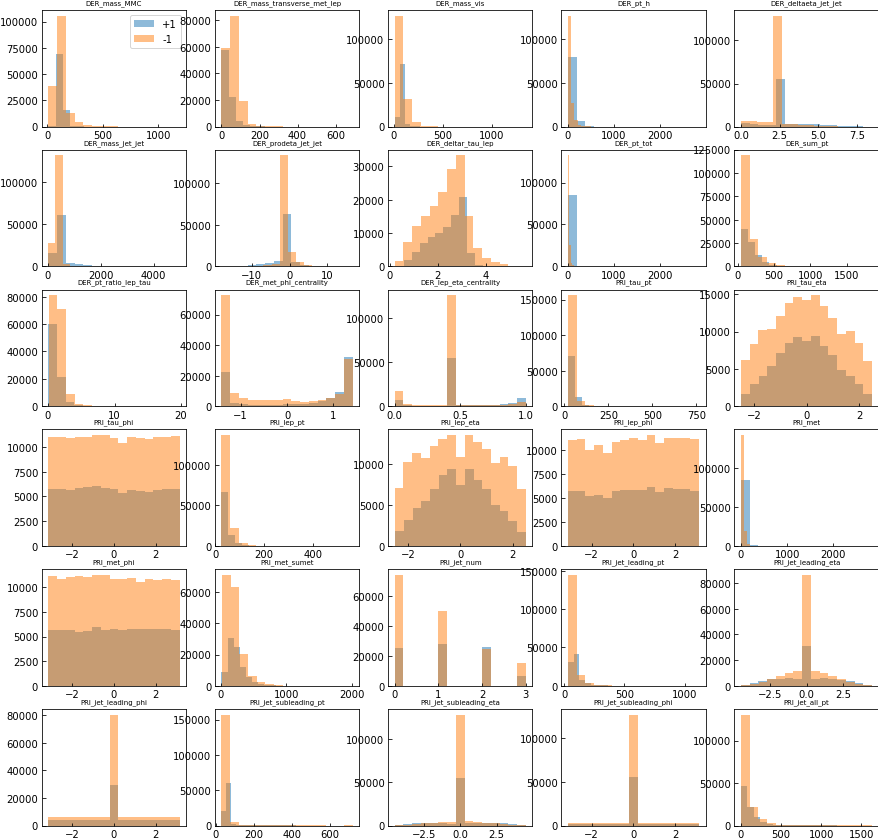
\includegraphics[width=100px]{../src/analysis/xy_tr_imp}
	\centering 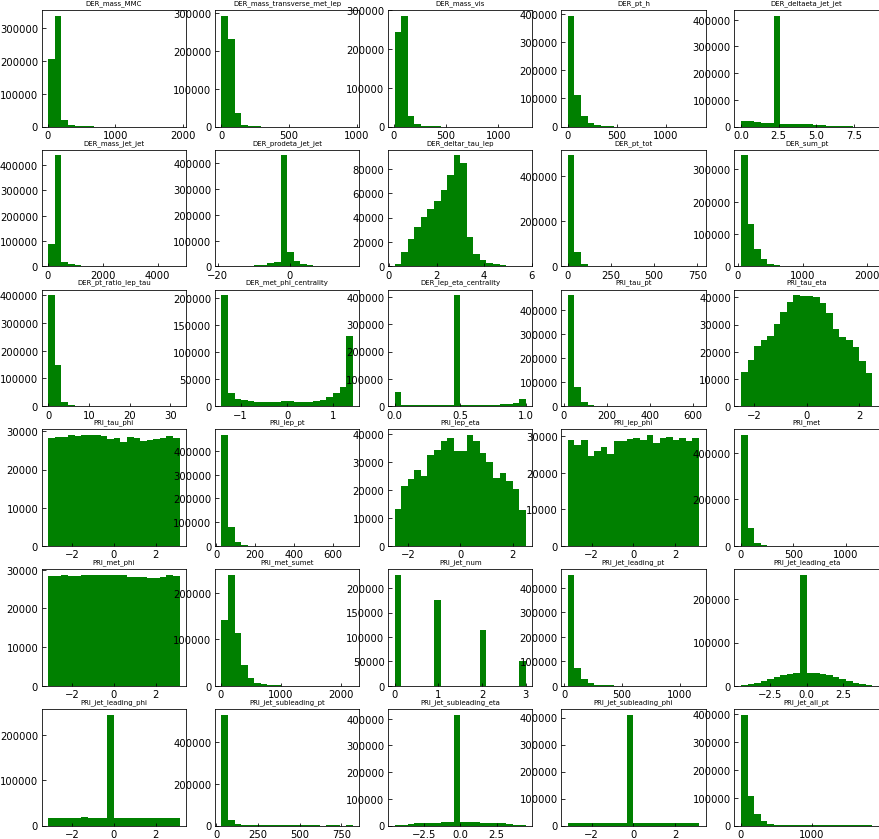
\includegraphics[width=100px]{../src/analysis/hist_te_imp}
	\centering 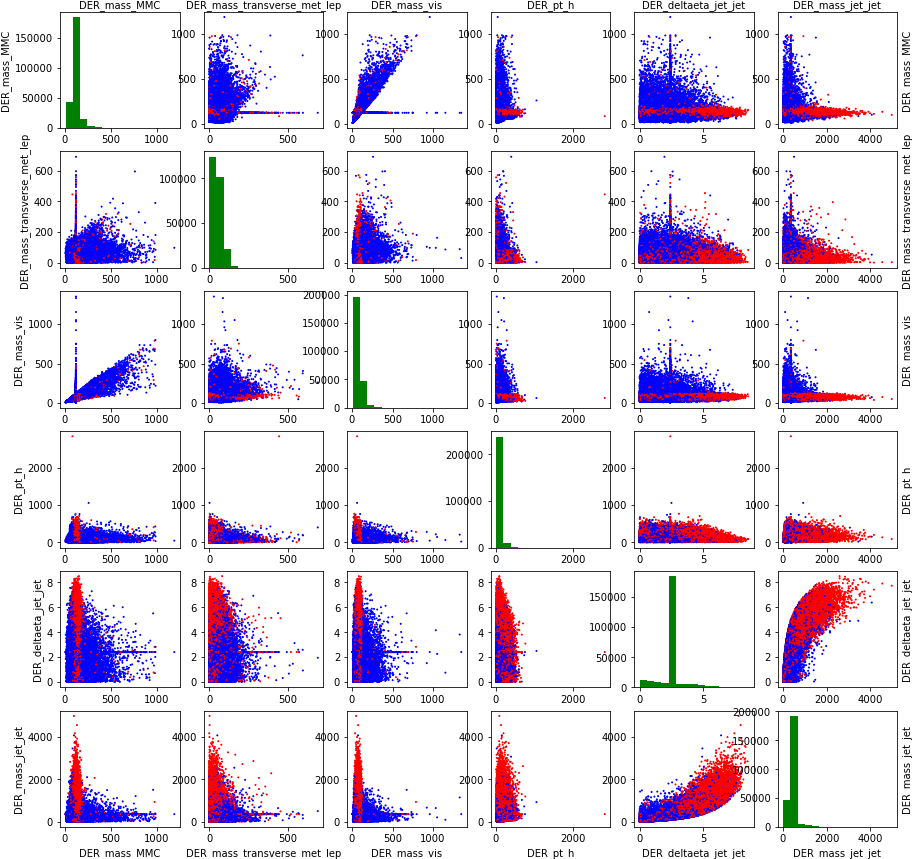
\includegraphics[width=100px]{../src/analysis/hist-scatter-tr-imp-0}
	\centering 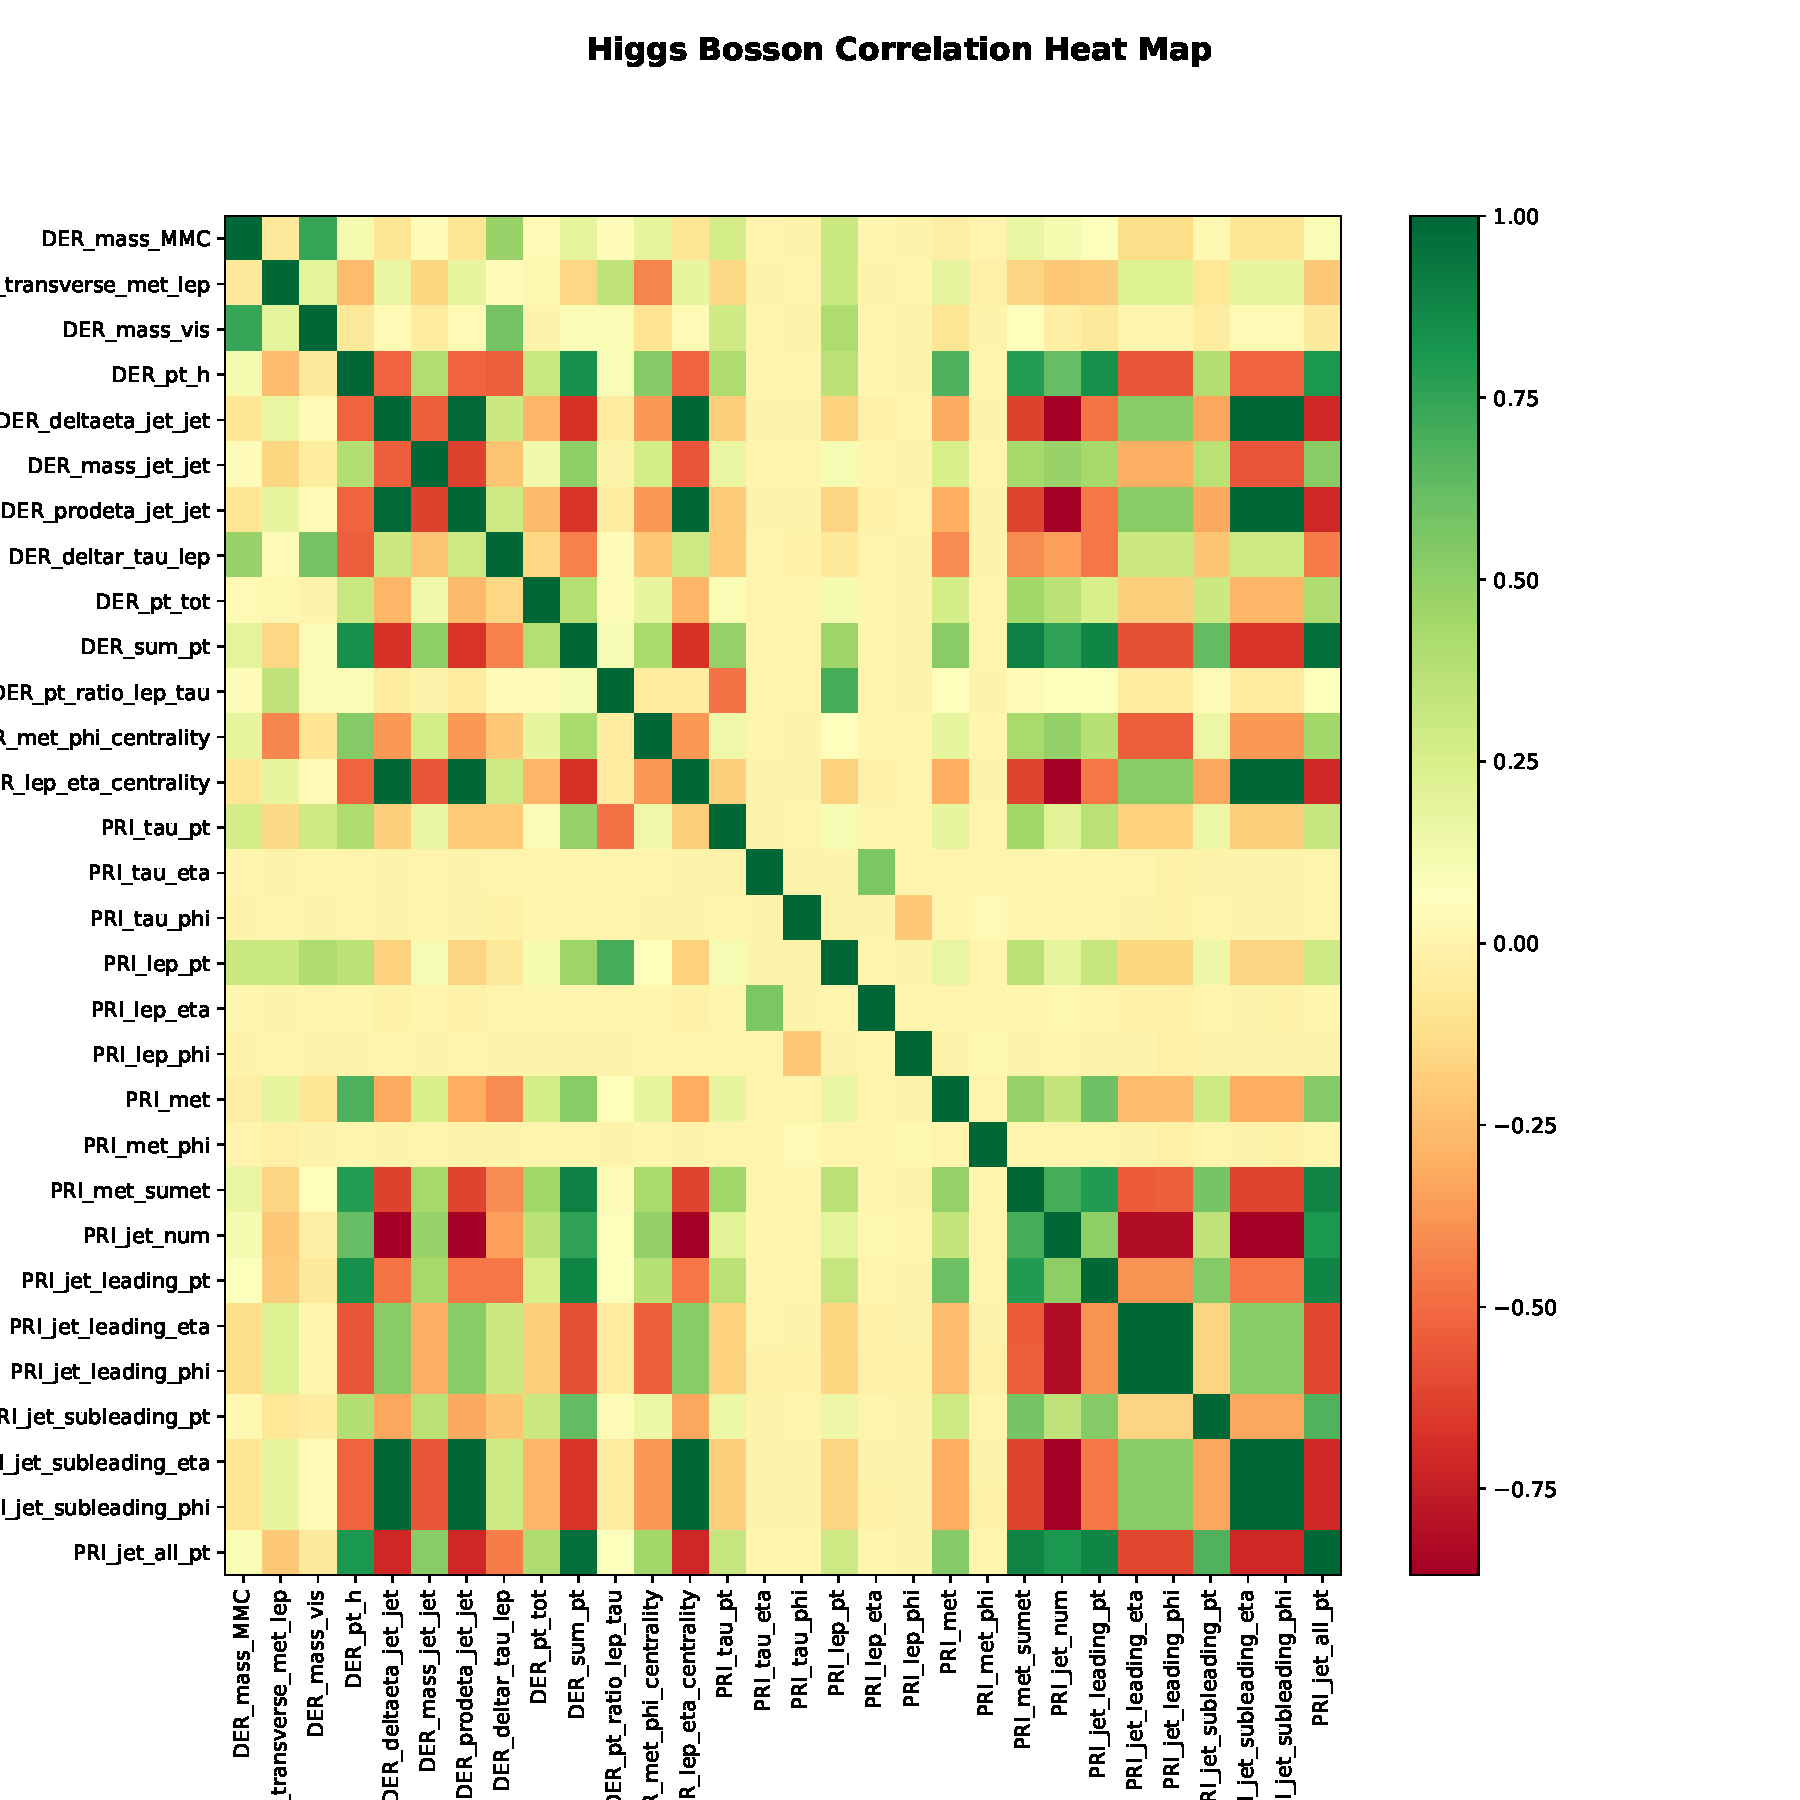
\includegraphics[width=100px]{../src/analysis/correlation}
	\caption{Exploratory data analysis using charts}
	\label{fig:data}
\end{figure}

First, the exploratory data analysis shows that most of the features (except one) are real-valued \ref{fig:data}, 1-2. Moreover, it is also can be seen that the test distribution does not differ from the train one \ref{fig:data}, 1. Scatter plots \ref{fig:data}, 3 show dependencies between features, as well as the correlation plot \ref{fig:data}, 4.

To begin with, a simple linear regression model is used on raw data (with a constant feature added), with 5-fold cross-validation to control overfitting. The results of each subsample are averaged to provide train/test accuracy. However, the model gives unsatisfying results on the hold-out dataset. As a means to deal with this issue, feature imputation and feature engineering is used: missing features are imputed with mean values (and `missing value` feature is added), categorical features are binarized. Moreover, it has been discovered that some of the features represent particle's mass, momentum or energy. Using the fact that squaring these quantities would make linear combinations of them meaningful in terms of physics ($E^2=m^2+p^2$), we introduce the polynomial basis. Table \ref{tab:feature_proc} shows the respective effects of these tricks.

\begin{figure}[!htb]
	\centering 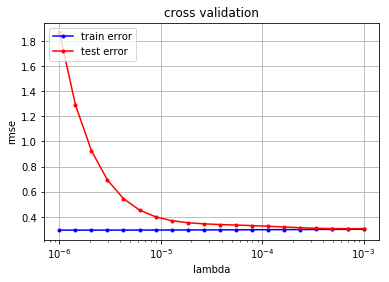
\includegraphics[width=110px]{linear_5}
	\centering 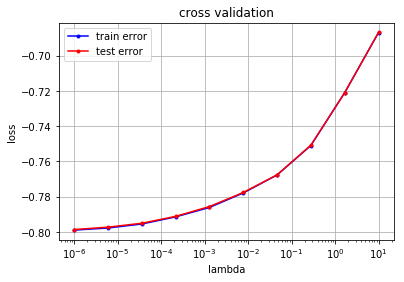
\includegraphics[width=110px]{ridge_accuracy_deg6}
	\caption{Degree 6 basis, MSE and Accuracy metrics}
	\label{fig:deg6}
\end{figure}

Applying ridge regression, it might be seen that it does not overfit in terms of accuracy (but does in terms of MSE \ref{fig:deg6}) on the dataset given even for the 6th degree, meaning that there is no significant difference between the test and the train accuracies. Applying it for different degrees, one obtains results shown in the Table \ref{tab:degrees}. It can be seen that 

\section{Models and Methods}
\begin{table}[!htb]
	\caption{Polynomial basis and linear regression, $\lambda=0$}	\label{tab:degrees}
	\centering\begin{tabular}{|lcccc|}\hline
		{\bf Degree} & {\bf Test accuracy} & {\bf MSE Test} & {\bf MSE Train} & {$\lambda$ best}\\
		1 & 0.7470 & 0.3378 & 0.3377 & $10^{-6}$\\
		2 & 0.7737 & 0.3483 & 0.3158 & $10^{-2}$\\		
		3 & 0.7850 & 0.3060 & 0.3040 & $10^{-4}$\\
		4 & 0.7937 & 0.3030 & 0.3010 & 0.0004\\
		5 & 0.7971 & 0.3050 & 0.3010 & 0.0006\\\hline
	\end{tabular}
\end{table}

As can be seen in the figures and results, while train MSE is continuously decreasing because of over-fitting, there is no significant change in test error after third degree polynomial basis. Therefore, feature extraction using polynomial basis does not seem to work for higher degrees. Furthermore, the accuracy of the model in Kaggle is not as good as what we expected (below 0.8), so that we decided to switch logistic regression since it uses a loss function tailored for the purpose of classification.

Applying logistic regression to the dataset, we have found out that it is crucial to implement the Newton's method since gradient update rule is taking too much time since final iterations are going with a small step size. Moreover, we discovered that the magnitude $\gamma$ of the gradient step depends on the size of the dataset. Therefore, we use batched version of stochastic gradient descent for logistic regression as the optimizer to stabilize the size of the dataset the optimizer uses for training.
However, applying this batched version to the dataset was costly due to the fact that working with a large matrix in numpy is faster than working with $k$ smaller matrices. Therefore, we used the standard Netwon algorithm and tuned the $\gamma$ manually for the final model.

The Figure \ref{fig:logreg}, 1 shows logistic regression accuracy for different regularization parameters $\lambda$. For this experiment, a constant number of iterations $20$ was chosen. The $\gamma$ parameter equals $\gamma=10^{-1}$. The chart indicates that the logistic regression does not overfit. Therefore, we have chosen the first in magnitude value of $\lambda=2\times 10^{-4}$ which allowed us to use $\gamma=0.1$ without overflows in loss. The figure \ref{fig:logreg}, 2 indicates the training schedule. Total number of $N=70$ iterations allowed us to bring the training error to 0. The solution has scored 0.82058 on Kaggle \cite{kaggle} (first part of test).

Despite the fact that the gradient at the final point was close to $0$ compared to the previous values, the value of the loss did not equal to 0. Moreover, it can be seen that the train and test errors ware similar. These two facts indicate that linear model has a high bias and low variance when applied to this dataset.

\begin{figure}[!htb]
	\centering 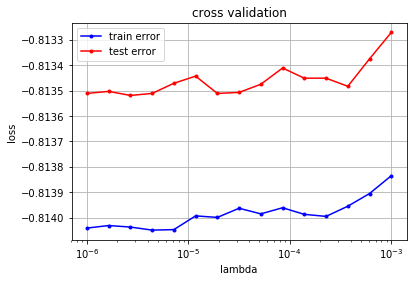
\includegraphics[width=150px]{logistic_lambda_cv_netwon_nobatch}
	\centering 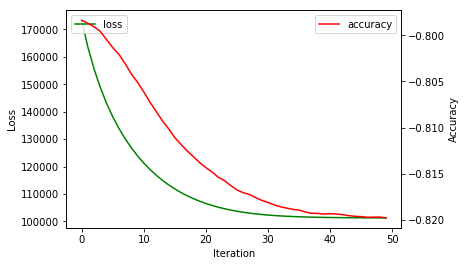
\includegraphics[width=150px]{logistic_01}
%	\centering 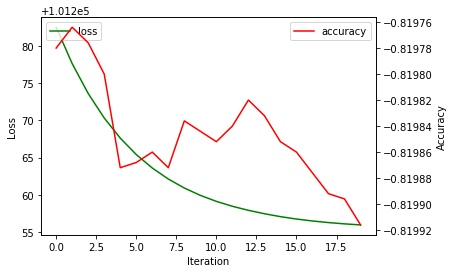
\includegraphics[width=200px]{logistic_02}
	
	\caption{Degree 5 basis, Logistic regression accuracy}
	\label{fig:logreg}
\end{figure}

\section{Results}
We have presented an application of linear, ridge and logistic regression to the dataset. The best model was logistic regression with best accuracy of 0.82 trained with Newton's method. All of the linear models do not overfit on the dataset.
\section{Discussion}
Despite thorough analysis, our project lacks further consideration in the following directions. First, it can be seen that some of the features do not look alike the Gaussian distribution. It might prove beneficial to split such features into two using a certain threshold. Moreover, it might be useful to apply boosting or bagging techniques, as well as to use more sophisticated nonlinear classifiers, such as neural networks.
\section{Summary}
We have shown that it is possible to detect the Higgs boson using linear methods and feature augmentation. Such a simple solution gives fairly good performance and places the team below average on the Kaggle submission. However, this approach is not optimal in terms of model selection, since a linear model seem to not capture all of the specifics of data since it produces high bias.
\begin{thebibliography}{99}
\bibitem{higgs} \href{https://en.wikipedia.org/wiki/Higgs\_boson}{en.wikipedia.org/wiki/Higgs\_boson}
\bibitem{data} \href{http://higgsml.lal.in2p3.fr/files/2014/04/documentation\_v1.8.pdf}{Experiment and feature description}
\bibitem{kaggle} \href{http://kaggle.com/c/epfml-higgs}{EPFL ML Project 1}
\end{thebibliography}

\end{document}
